\chapter{Marco Teórico}

\section{Series Temporales}

Una serie temporal es una secuencia de observaciones $\{y_t\}_{t=1}^{T}$ indexadas en el tiempo, donde el orden de las observaciones es la parte esencial. A diferencia de los datos de corte transversal, en una serie temporal la dependencia entre observaciones consecutivas constituye la principal fuente de información para las predicciones. 

Formalmente, se asume que cada observación $y_t$ es una realización de una variable aleatoria $Y_t$, y el conjunto $\{Y_t\}_{t \in \mathbb{Z}}$ define un proceso estocástico. El objetivo del forecasting es estimar la distribución condicional:
$$p(Y_{t+h} \mid \mathcal{F}_t),$$
donde $h \geq 1$ es el horizonte de predicción y $\mathcal{F}_t = \sigma(Y_t, Y_{t-1}, ...)$ es la filtración generada por la historia del proceso hasta el tiempo $t$. En la práctica, la mayoría de los modelos de forecasting estiman únicamente la media condicional $\mathbb{E}[Y_{t+h} \mid \mathcal{F}_t]$, produciendo predicciones puntuales. Sin embargo, para la toma de decisiones bajo incertidumbre, como la programación del despacho eléctrico o valorización de contratos en el SEN, es necesario tener garantías estadísticas con respecto a las predicciones.

\subsection{Estacionariedad}

Un proceso estocástico $\{Y_t\}$ se denomina estrictamente estacionario si su distribución conjunta es invariante ante traslaciones temporales, es decir, si para todo $k \in \mathbb{Z}$ y todo conjunto finito de índices $\{t_1, \ldots, t_n\}$ se cumple que:

\begin{equation}
    (Y_{t_1}, \ldots, Y_{t_n}) \overset{d}{=} (Y_{t_1+k}, \ldots, Y_{t_n+k})
\end{equation}

La estacionariedad es una propiedad estructural de un proceso estocástico que describe la invarianza de sus características estadísticas en el tiempo. En la práctica se trabaja con la noción más débil de \textit{estacionariedad en covarianza} o \textit{estacionariedad débil}, que exige únicamente que:

\begin{align*}
    \mathbb{E}[Y_t] &= \mu \quad \forall\, t\geq 0 \\
    \text{Cov}(Y_t, Y_{t+k}) &= \gamma(k) \quad \forall\, t, k \geq 0
\end{align*}

La estacionariedad es un supuesto central en los modelos estadísticos clásicos como ARIMA, cuya validez depende de que la serie no muestre tendencias ni cambios estructurales en su nivel de varianza. En mercados eléctricos con alta penetración renovable, es frecuente observar no estacionariedad de múltiples orígenes: tendencias de largo plazo asociadas a cambios estructurales en la matriz energética, heterocedasticidad vinculada a episodios de sobreoferta, y quiebres abruptos por eventos hidrológicos o de congestión.

Un proceso no estacionario que puede volverse estacionario mediante diferenciación de orden $d$ se denomina integrado de orden $d$, denotado $I(d)$. La verificación formal de este supuesto se realiza mediante pruebas de raíz unitaria. La prueba \textit{Augmented Dickey-Fuller} (ADF) contrasta la hipótesis nula de raíz unitaria contra la alternativa de estacionariedad, mientras que la prueba \textit{KPSS} invierte el rol de las hipótesis, contrastando estacionariedad como hipótesis nula. El uso conjunto de ambas pruebas permite una caracterización más robusta de la estructura de la serie.

\begin{figure}[htbp]
    \centering
    \begin{subfigure}[b]{0.48\textwidth}
        \centering
        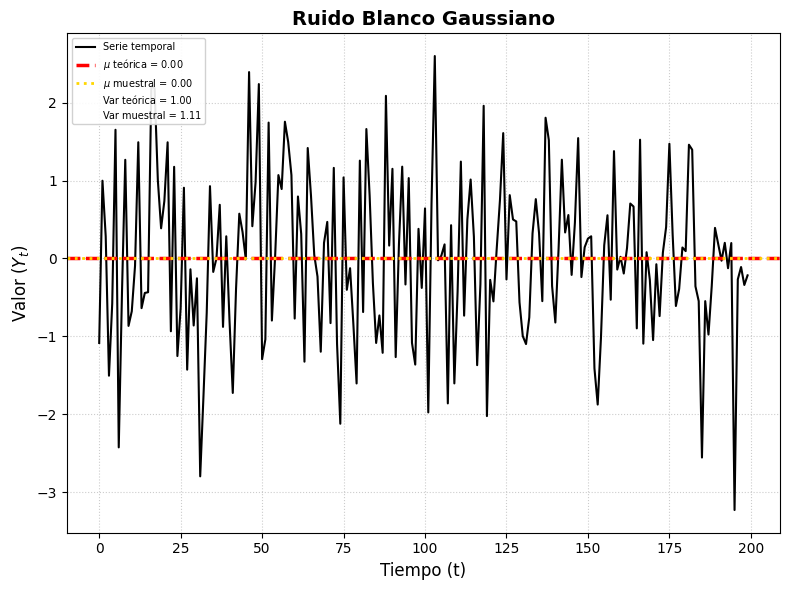
\includegraphics[width=\textwidth]{imagenes/Posibles img/Ruido Blanco.png}
        \caption{Serie Estacionaria ($\mu$ y $\sigma$ constantes)}
        \label{fig:estacionaria}
    \end{subfigure}
    \hfill
    \begin{subfigure}[b]{0.48\textwidth}
        \centering
        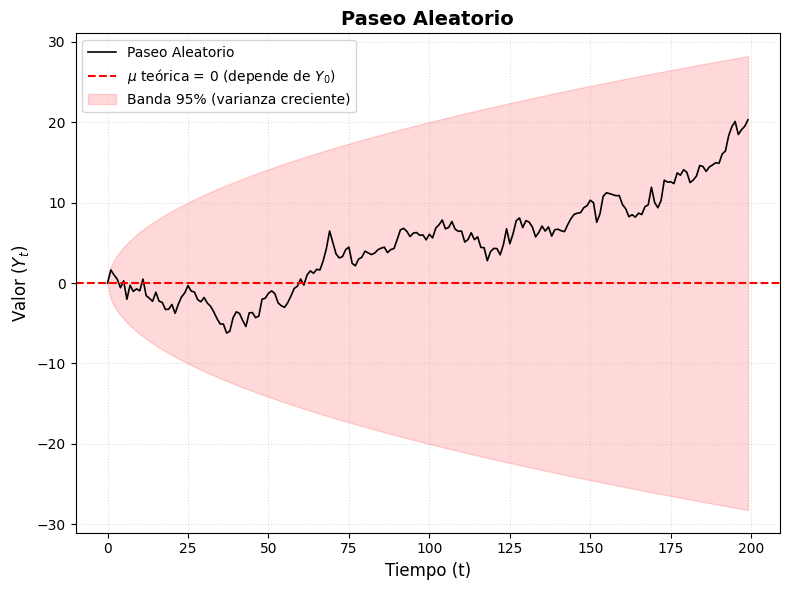
\includegraphics[width=\textwidth]{imagenes/Posibles img/Paseo Aleatorio.png}
        \caption{Serie No Estacionaria($\mu$ y $\sigma$ variables)}
        \label{fig:no_estacionaria}
    \end{subfigure}
    \caption{Ejemplificación de una serie estacionaria y una no estacionarias.}
    \label{fig:comparacion_series}
\end{figure}

\subsection{Estacionalidad múltiple}

Una serie temporal exhibe estacionalidad cuando presenta patrones que se repiten con una periodicidad fija $m$. En el contexto de series temporales de precios eléctricos, es habitual observar estacionalidad en múltiples escalas simultáneamente: un patrón diario de periodo $m_1=24$ horas, asociado al ciclo de demanda residencial e industrial, un patrón semanal de periodo $m_2=168$ horas, determinado por la diferencia entre días hábiles y fines de semana, y un patrón anual de periodo $m_3=8760$ horas, vinculado a la variación estacional de la radiación solar y la hidrología.

La manera natural de modelar esta estructura es mediante una descomposición aditiva:

\begin{equation}
    y_t = T_t + \sum_{j=1}^{J} S_t^{(j)} + \varepsilon_t\quad,
\end{equation}

donde $T_t$ es la componente de tendencia, $S_t^{(j)}$ es la $j$-ésima componente estacional de periodo $m_j$ y $\varepsilon_t \sim \mathcal{N}(0, \sigma^2)$ es el término de error. La idea de este modelo radica en el supuesto de que las fuentes de variación son conceptualmente separables y aditivas: la tendencia captura la dinámica de largo plazo del mercado, cada componente estacional captura un ciclo recurrente de distinta escala, y el residuo recoge la variabilidad no estructurada.

En el contexto de series temporales, una componente estacional $S_t^{(j)}$ de periodo $m$ es por definición una función periódica, por lo que puede representarse mediante una serie de Fourier truncada de orden $K_j$:

\begin{equation}
    S_t^{(j)} = \sum_{k=1}^{K_j} \left[ a_k^{(j)} \cos\left(\frac{2\pi k t}{m_j}\right) + b_k^{(j)} \sin\left(\frac{2\pi k t}{m_j}\right) \right]
    \label{eq:fourier_seasonality}
\end{equation}

donde los coeficientes $\{a_k^{(j)}, b_k^{(j)}\}$ son parámetros estimables. Esta representación viene de la teoría clásica de señales, donde cualquier función periódica de periodo $m$ que sea integrable puede aproximarse mediante sumas de senos y cosenos de frecuencias múltiplos de $\frac{1}{m}$.

Esta representación tiene tres ventajas que la hacen adecuada para su estimación mediante optimización:es diferenciable, lo que permite la optimización por descenso de gradiente, es flexible, pues puede aproximar estacionalidades de cualquier forma y no solo senoidales, y parsimoniosa, lo que permite capturar patrones complejos con pocos coeficientes. El orden $K_j$ controla la suavidad de la estacionalidad estimada: valores pequeños de $K_j$ producen componentes suaves, mientras que valores grandes permiten capturar formas más irregulares.

\begin{figure}[htbp]
    \centering
    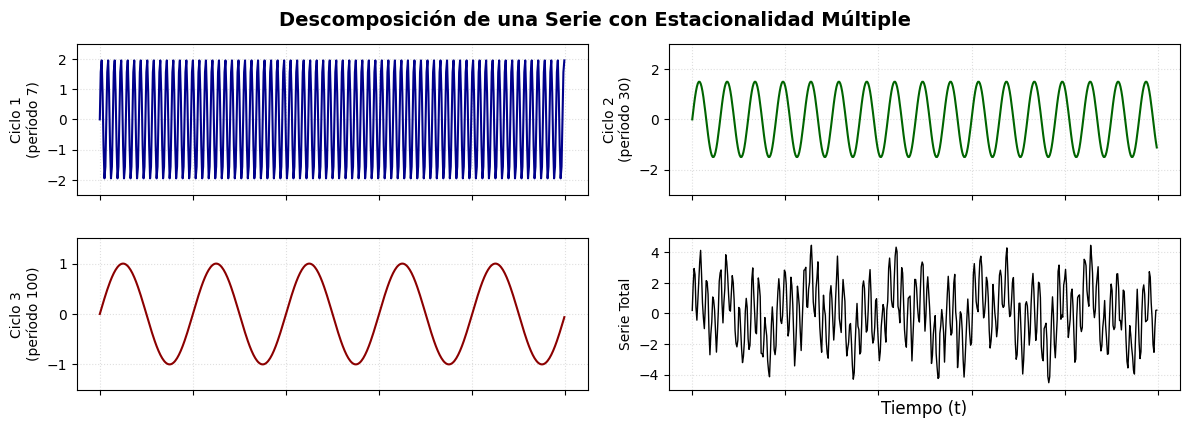
\includegraphics[width=0.9\linewidth]{imagenes/Posibles img/Estacionalidad.png}
    \caption{Visualización de una serie con estacionalidad múltiple descompuesta}
    \label{fig:placeholder}
\end{figure}

\subsection{Procesos no estacionarios y transformaciones}

Cuando una serie presenta tendencia, varianza no constante o cambios estructurales, es necesario aplicar transformaciones previas al entrenamiento para estabilizar sus propiedades estadísticas y mejorar la convergencia de los modelos. La transformación más utilizada en el contexto de modelos de aprendizaje profundo es la \textit{estandarización} o \textit{normalización z-score}, que transforma cada observación según:

\begin{equation}
    \tilde{y}_t = \frac{y_t - \hat{\mu}}{\hat{\sigma}}
\end{equation}

donde $\hat{\mu}$ y $\hat{\sigma}$ son la media y desviación estándar estimadas exclusivamente sobre el conjunto de entrenamiento. Esta transformación garantiza que la serie transformada tenga media cero y varianza unitaria, lo que estabiliza el gradiente durante el entrenamiento y hace que los parámetros del modelo sean comparables entre distintas barras y horizontes. Es fundamental que los parámetros $\hat{\mu}$ y $\hat{\sigma}$ se estimen solo sobre el conjunto de entrenamiento y se apliquen sin reestimación al conjunto de validación y prueba, evitando así la filtración de información futura o \textit{data leakage}. 

Otras transformaciones comunes en la literatura incluyen la diferenciación de orden $d$, que elimina tendencias polinomiales, y la transformación logarítmica, que estabiliza la varianza en series con heterocedasticidad multiplicativa. En este trabajo se adopta la estandarización z-score como transformación principal, aplicada de manera independiente a cada barra del SEN mediante \texttt{StandardScaler}.

\subsection{Horizonte de predicción y estrategia de forecasting multihorizonte}

El horizonte de predicción $h$ determina cuántos pasos adelante se desea predecir. En mercados eléctricos, el horizonte más relevante operacionalmente es el \textit{day-ahead}, es decir, $h=24$ horas, que corresponde al ciclo de programación del despacho en el SEN. En este trabajo se adopta un horizonte de $h=1$ hora, lo que corresponde a la predicción del costo marginal de la hora inmediata siguiente dado una ventana de predicción de longitud $L$. Formalmente, el problema de predicción se define como estimar:

\begin{equation}
    \hat{y}_{t+1} = f\left(y_{t-L+1:t},\, \mathbf{x}_{t-L+1:t+1}\right)
\end{equation}

donde $L$ es la longitud de la ventana de contexto y $\mathbf{x}_t$ denota el vector de covariables exógenas conocidas en el tiempo $t$, como temperatura, demanda o generación, y $f$ es el modelo de forecasting.

Aunque en este trabajo se considera $h=1$, vale la pena situar este caso dentro del marco general de estrategias de forecasting multihorizonte, dado que el TFT fue diseñado para el caso general $h \geq 1$. Las tres estrategias principales son: la estrategia \textit{recursiva}, que aplica iterativamente el modelo de un paso para generar predicciones de múltiples horizontes usando predicciones previas como entrada; la estrategia \textit{directa}, que entrena un modelo independiente para cada horizonte $h$, y la estrategia MIMO (\textit{Multiple Input Multiple Output}), que predice simultáneamente todos los horizontes con un único modelo, capturando las dependencias entre ellos. El TFT adopta la estrategia MIMO, lo que lo hace naturalmente extensible a horizontes mayores si el alcance del trabajo lo permite.

Un concepto distinto pero relacionado con el horizonte de predicción es la \textit{granularidad} o resolución temporal de la serie, es decir, el intervalo de muestreo entre observaciones consecutivas. Mientras el horizonte $h$ determina cuántos pasos futuros se predicen, la granularidad determina la duración real de cada paso: una serie horaria y una serie de 15 minutos pueden compartir el mismo horizonte $h=1$ en número de pasos, pero constituyen problemas de predicción distintos, con distinta cantidad de observaciones por unidad de tiempo y, potencialmente, distinta relación señal-ruido en la ventana de contexto $L$. El pipeline principal de este trabajo se construye sobre datos horarios, resolución que coincide con el ciclo de programación y liquidación del costo marginal en el SEN; el Capítulo 4 explora de manera preliminar el efecto de contrastar esta resolución con series diarias y de 15 minutos sobre el desempeño del modelo.

\subsection{Forecasting multivariado y estructura de barras}

En este trabajo el problema de forecasting no se limita a una única serie, sino que se extiende a $B = 8$ barras del SEN, cada una con su propia serie de costos marginales horarios$\{y_t^{(b)}\}_{t=1}^{T} \, \text{con} \quad b=1, ...,8$. Este escenario define un problema de forecasting multivariado, donde las series pueden presentar dependencias cruzadas, por ejemplo, barras eléctricamente contiguas tienden a exhibir costos marginales correlacionados, salvo en episodios de congestión de transmisión, donde los precios se desacoplan, generando heterogeneidad estructural entre barras. 

Esta correlación entre barras puede cuantificarse formalmente mediante una función de correlación cruzada, lo que en principio permitiría un enfoque de \textit{forecasting con dependencias espaciales}, donde la predicción para la barra $b$ incorpora información de las barras vecinas. Sin embargo, este enfoque requiere modelar explícitamente la topología de la red eléctrica y puede introducir complejidad adicional cuando las congestiones generan desacoplamientos no estacionarios entre barras.

La estrategia adoptada en este trabajo consiste en entrenar un modelo independiente por barra, lo cual simplifica el problema a costa de ignorar las dependencias cruzadas. Esta decisión se justifica por dos razones: las congestiones de transmisión en el SEN introducen heterogeneidad estructural entre barras que dificultaría el entrenamiento conjunto, y los modelos independientes son más interpretables y permiten identificar con claridad el comportamiento especifico de cada barra. La incorporación de dependencias espaciales mediante correlación cruzada queda propuesta como una extensión natural de este trabajo para investigación futura.

\section{Prophet}

Prophet es un modelo de \textit{forecasting} de series temporales desarrollado por Taylor y Letham (2018) en Meta \cite{Prophet}, diseñado para producir predicciones interpretables en series con patrones estacionales fuertes, valores faltantes (\textit{missing values}) y cambios de tendencia abruptos. A diferencia de los modelos estadísticos clásicos como ARIMA y sus variantes, Prophet no requiere que la serie sea estacionaria ni impone supuestos sobre la estructura de autocorrelación de los residuos. Su diseño está orientado a la estimación automática de componentes interpretables, lo que lo hace especialmente adecuado como componente de descomposición en arquitecturas híbridas.

Prophet formula el problema de forecasting como la estimación de un modelo aditivo de la forma:

\begin{equation}
\hat{y}_t^{Prophet} = T(t) + S(t) + H(t) + \varepsilon_t
\end{equation}

donde $T(t)$ es la componente de tendencia, $S(t)$ es la componente de estacionalidad, $H(t)$ captura el efecto de días festivos y eventos especiales, y $\varepsilon_t \sim \mathcal{N}(0, \sigma^2)$ es el término de error. Cada componente se estima de manera independiente, lo que otorga al modelo su interpretabilidad característica. La estimación de los parámetros se realiza mediante inferencia bayesiana con el software Stan, lo que permite incorporar incertidumbre en las predicciones de manera natural.

\subsection{Componente de tendencia}

Prophet ofrece dos especificaciones para la componente de tendencia $T(t)$. La primera es un \textit{modelo de crecimiento logístico}, adecuado para trabajar con series que tienen un capacidad máxima o saturación:

\begin{equation}
T(t) = \frac{C}{1 + e^{-k(t - m)}}
\end{equation}

donde $C$ es la capacidad de saturación, $k$ es la tasa de crecimiento y $m$ es el punto de inflexión. La segunda, y más utilizada en series de precios, es un \textit{modelo lineal por tramos} (\textit{piecewise linear}):

\begin{equation}
T(t) = (k + \mathbf{a}(t)^\top \boldsymbol{\delta})t + (m + \mathbf{a}(t)^\top \boldsymbol{\gamma})
\end{equation}

donde $k$ es la tasa de crecimiento global, $\boldsymbol{\delta} \in \mathbb{R}^S$ es el vector de cambios de pendiente en cada uno de los $S$ puntos de quiebre, $\mathbf{a}(t) \in \{0,1\}^S$ es un vector indicador que activa los cambios acumulados hasta el tiempo $t$, y $\boldsymbol{\gamma}$ ajusta el intercepto para garantizar continuidad en los puntos de quiebre. Los puntos de quiebre pueden especificarse manualmente o detectarse automáticamente por el modelo, lo que le permite adaptarse a cambios estructurales graduales como los que experimenta el costo marginal del SEN ante la incorporación continua de capacidad renovable.

La detección automática de los puntos de quiebre se realiza colocando una distribución a priori dispersa sobre los ajustes de pendiente $\boldsymbol{\delta} \sim \text{Laplace}(0, \tau)$, donde $\tau > 0$ controla la flexibilidad del modelo. Un prior disperso permite que Prophet proponga un gran número de puntos de quiebre candidatos, típicamente uno por mes en una historia de varios años, pero penaliza aquellos ajustes que no son necesarios para explicar los datos. Cuando $\tau \to 0$, el modelo reduce a una tendencia lineal o logística simple sin quiebres. Este mecanismo de regularización es especialmente relevante para las series de costos marginales del SEN, donde los cambios estructurales son graduales y difíciles de datar con precisión \cite{Prophet}.

\subsection{Componente de estacionalidad}

La componente estacional $S(t)$ se modela como la suma de las componentes de Fourier truncadas $S_t^{(j)}$ de la Ecuación \eqref{eq:fourier_seasonality} (Sección 2.1.2) sobre las $J$ escalas estacionales consideradas, $S(t) = \sum_{j=1}^{J} S_t^{(j)}$. El orden $K_j$ controla la flexibilidad de cada componente estacional: Prophet usa por defecto $K=10$ para la estacionalidad anual y $K=3$ para la semanal, valores que pueden ajustarse según la complejidad de los patrones observados. En este trabajo se consideran las estacionalidades diaria ($m_1 = 24$), semanal ($m_2 = 168$) y anual ($m_3 = 8760$), capturando los tres ciclos recurrentes identificados en la Sección 2.1.

\subsection{Componente de festividades y eventos especiales}

La componente $H(t)$ modela el efecto de días festivos y eventos especiales que producen desviaciones sistemáticas en la serie, no capturables por la estacionalidad regular. Prophet representa este efecto como:

\begin{equation}
H(t) = \mathbf{Z}(t)\boldsymbol{\kappa}
\end{equation}

donde $\mathbf{Z}(t) \in \{0,1\}^{L}$ es un vector indicador que activa el evento correspondiente al tiempo $t$, y $\boldsymbol{\kappa} \in \mathbb{R}^{L}$ es el vector de efectos estimados para cada uno de los $L$ eventos definidos. En este trabajo se incorporan los feriados nacionales del calendario chileno, dado que el consumo eléctrico y el despacho del SEN exhiben patrones sistemáticamente distintos en días festivos respecto a días hábiles.

\subsection{Estimación e inferencia}

Análogamente al prior sobre el cambio de tendencia $\boldsymbol{\delta}$ (Sección 2.2.1), los coeficientes estacionales reciben una distribución a priori $\boldsymbol{\beta} \sim \mathcal{N}(0, \sigma_s^2)$, donde $\sigma_s$ es el hiperparámetro \texttt{seasonality\_prior\_scale} que regula la flexibilidad de la estacionalidad, ajustado por barra junto con $\tau$ en la Sección 3.3.1. La inferencia se realiza mediante \textit{Maximum A Posteriori} (MAP), suficiente para los fines de este trabajo dado que la cuantificación de incertidumbre de las predicciones finales se aborda mediante el TFT y Conformal Prediction (Secciones 2.3.4 y 2.6), y no mediante los intervalos de credibilidad bayesianos de Prophet.

\subsection{Rol de Prophet en la arquitectura híbrida}

En el modelo propuesto en este trabajo, Prophet cumple el rol de componente de descomposición temporal. Dado que Prophet modela explícitamente la tendencia, la estacionalidad múltiple y los efectos de calendario, sus predicciones capturan la estructura sistemática de largo plazo de la serie. Los residuos de Prophet:

\begin{equation}
r_t = y_t - \hat{y}_t^{\text{Prophet}}
\end{equation}

representan la variabilidad no explicada por la estructura sistemática, episodios de sobreoferta renovable, congestiones de transmisión y fluctuaciones de corto plazo, que son precisamente las componentes que el TFT está mejor equipado para modelar. Esta separación de roles motiva el diseño de dos modelos TFT paralelos: uno entrenado sobre los residuos $\{r_t\}$ y otro entrenado directamente sobre la serie original $\{y_t\}$, las predicciones se combinan con las hechas por Prophet posteriormente mediante Stacking Optimization, como se detalla en la Sección 2.5.

Esta descripción corresponde específicamente a la rama \textbf{Prophet+Clima (P+C)} del modelo propuesto en este trabajo. La Sección 2.3.5 presenta el rol del TFT dentro de esta rama junto con el de la rama alternativa \textbf{Sol+Clima (S+C)}, que prescinde por completo de Prophet.

\section{Transformer y Temporal Fusion Transformer}

El mecanismo de atención y la arquitectura Transformer, introducidas por Vaswani et al. (2017) \cite{Vaswani2017Attention} revolucionaron el procesamiento secuencial de datos y el \textit{Deep Learning}. Hasta entonces, los dos paradigmas dominantes para el modelado de secuencias eran las arquitecturas recurrentes, en particular las \textit{Redes Neuronales Recurrentes} (RNN) y los modelos de \textit{Memoria Larga a Corto Plazo} (LSTM), y las arquitecturas convolucionales aplicadas a secuencias. Ambas familias presentaban limitaciones complementarias: las recurrentes procesaban la secuencia de forma inherentemente secuencial, lo que impedía su paralelización durante el entrenamiento, mientras que las convolucionales, aunque paralelizables, requerían apilar múltiples capas para capturar dependencias de largo alcance. El Transformer elimina simultáneamente la recurrencia y la convolución, reemplazándolas por un mecanismo de auto-atención que conecta cualquier par de posiciones de la secuencia en un número constante de operaciones, permitiendo tanto la paralelización completa del entrenamiento como el modelado directo de dependencias de largo alcance \cite{Vaswani2017Attention}. En esta sección se presenta primero el mecanismo de atención y la arquitectura Transformer clásica, para luego describir el \textit{Temporal Fusion Transformer} (TFT), la variante especializada para forecasting multihorizonte utilizada en este trabajo.

\subsection{Mecanismo de atención}

El mecanismo de atención permite que un modelo pondere diferencialmente la relevancia de distintas posiciones de una secuencia al producir una representación para cada posición. La idea central es que, al predecir el valor en el tiempo $t$, no todas las observaciones pasadas son igual de relevantes, algunas tienen mayor influencia que otras dependiendo del contexto.

Formalmente, el mecanismo de atención opera sobre tres matrices: las \textit{queries} $\mathbf{Q} \in \mathbb{R}^{n \times d_k}$, las \textit{keys} $\mathbf{K} \in \mathbb{R}^{m \times d_k}$ y los \textit{values} $\mathbf{V} \in \mathbb{R}^{m \times d_v}$, donde $n$ es el número de posiciones de consulta, $m$ el número de posiciones de referencia, $d_k$ la dimensión de las queries y keys, y $d_v$ la dimensión de los values. La salida del mecanismo de atención es:

\begin{equation}
\text{Attention}(\mathbf{Q}, \mathbf{K}, \mathbf{V}) = \text{softmax}\left(\frac{\mathbf{Q}\mathbf{K}^\top}{\sqrt{d_k}}\right)\mathbf{V}
\end{equation}

El término $\mathbf{Q}\mathbf{K}^\top \in \mathbb{R}^{n \times m}$ calcula los productos punto entre cada query y cada key, produciendo una matriz de \textit{scores} que mide la afinidad entre pares de posiciones. La división por $\sqrt{d_k}$ estabiliza los gradientes durante el entrenamiento: sin este factor, cuando $d_k$ es grande los productos punto crecen en magnitud y empujan a la función softmax hacia regiones de gradiente muy pequeño. La función softmax normaliza los \textit{scores} por filas, produciendo para cada posición una combinación convexa ponderada de los values de las posiciones de referencia. Este mecanismo se denomina \textit{scaled dot-product attention} y tiene complejidad computacional $\mathcal{O}(n \cdot m \cdot d_k)$ en tiempo y $\mathcal{O}(n \cdot m)$ en memoria, lo que puede ser restrictivo para secuencias largas.

\subsection{Atención multi-cabeza}

En la práctica, es beneficioso que el modelo pueda atender a distintos tipos de relaciones simultáneamente, por ejemplo, dependencias de corto plazo y de largo plazo al mismo tiempo. La \textit{atención multi-cabeza} (\textit{multi-head attention}) logra esto proyectando las queries, keys y values en $H$ subespacios distintos y calculando la atención en cada uno, de forma paralela:

\begin{equation}
\text{MultiHead}(\mathbf{Q}, \mathbf{K}, \mathbf{V}) = \text{Concat}(\text{head}_1, \ldots, \text{head}_H) \,\mathbf{W}^O
\end{equation}

donde cada cabeza se define como:

\begin{equation}
\text{head}_h = \text{Attention}(\mathbf{Q}\mathbf{W}_h^Q, \mathbf{K}\mathbf{W}_h^K, \mathbf{V}\mathbf{W}_h^V)
\end{equation}

con matrices de proyección $\mathbf{W}_h^Q \in \mathbb{R}^{d_{\text{model}} \times d_k}$, $ \mathbf{W}_h^K \in \mathbb{R}^{d_{\text{model}} \times d_k}$, $\mathbf{W}_h^V \in \mathbb{R}^{d_{\text{model}} \times d_v}$ y $\mathbf{W}^O \in \mathbb{R}^{H d_v \times d_{\text{model}}}$. Típicamente se fija $d_k = d_v = d_{\text{model}} / H$ para mantener el costo computacional equivalente al de una sola cabeza de dimensión completa.

\subsection{Arquitectura Transformer}

El Transformer completo apila $N$ bloques idénticos, alternando una capa de atención multi-cabeza y una red de alimentación directa (\textit{Feed-Forward Network}, FFN), ambas envueltas en conexiones residuales y normalización de capa, e incorpora una \textit{codificación posicional} (\textit{positional encoding}) senosoidal para inyectar el orden temporal de la secuencia, dado que el mecanismo de atención es en sí mismo invariante a permutaciones \cite{Vaswani2017Attention}. El Temporal Fusion Transformer, descrito en la Sección 2.3.4, se aparta de esta arquitectura genérica en dos aspectos centrales: reemplaza el bloque residual y la codificación posicional por una etapa de procesamiento secuencial local basada en LSTM (Sección 2.3.4.4), y sustituye la atención multi-cabeza estándar por un mecanismo de atención interpretable que comparte los values entre cabezas (Sección 2.3.4.6), conservando no obstante la formulación de \textit{queries}, \textit{keys} y \textit{values} presentada en esta sección.

\subsection{Temporal Fusion Transformer}

El Temporal Fusion Transformer (TFT), propuesto por Lim et al. (2021) \cite{TFT}, extiende la arquitectura Transformer para el problema específico de forecasting multihorizonte con covariables heterogéneas. A diferencia del Transformer clásico, el TFT incorpora mecanismos explícitos para el manejo de covariables estáticas, selección de variables relevantes, procesamiento secuencial local e interpretabilidad de las dependencias temporales aprendidas. La arquitectura se organiza en cinco componentes principales que se describen a continuación.

\subsubsection{Codificación de entradas y embeddings}

El TFT recibe tres tipos de entradas: covariables estáticas $\mathbf{s} \in \mathbb{R}^{d_s}$, que no varían en el tiempo, por ejemplo, el identificador de barra, covariables temporales pasadas conocidas $\mathbf{x}_{t-L:t} \in \mathbb{R}^{L \times d_x}$ y covariables temporales futuras conocidas $\mathbf{x}_{t:t+H} \in \mathbb{R}^{H \times d_x}$, por ejemplo, el día de la semana o el indicador de feriado. Cada variable es proyectada a un espacio de representación de dimensión $d_{\text{model}}$ mediante transformaciones lineales o embeddings aprendibles.

\subsubsection{Gated Residual Network}

El bloque fundamental del TFT es la \textit{Gated Residual Network} (GRN), que permite al modelo suprimir información irrelevante mediante una compuerta aprendible:

\begin{equation}
\text{GRN}(\mathbf{a}, \mathbf{c}) = \text{LayerNorm}\left(\mathbf{a} + \text{GLU}\left(\mathbf{W}_1 \, \text{ELU}(\mathbf{W}_2 \, \mathbf{a} + \mathbf{W}_3 \, \mathbf{c} + \mathbf{b}_2) + \mathbf{b}_1\right)\right)
\end{equation}

donde $\mathbf{a}$ es la entrada principal, $\mathbf{c}$ es un contexto opcional, ELU es la función de activación exponencial lineal, y GLU (\textit{Gated Linear Unit}) es el mecanismo de compuerta definido como:

\begin{equation}
\text{GLU}(\mathbf{h}) = \sigma(\mathbf{W}_4 \, \mathbf{h} + \mathbf{b}_3) \odot (\mathbf{W}_5 \, \mathbf{h} + \mathbf{b}_4)
\end{equation}

donde $\sigma$ es la función sigmoide y $\odot$ denota el producto de Hadamard. La compuerta $\sigma(\cdot)$ puede aprender a anular completamente la contribución del bloque cuando la entrada no es informativa, lo que dota al TFT de una capacidad de regularización adaptativa que el Transformer clásico no posee.

\subsubsection{Variable Selection Network}

La \textit{Variable Selection Network} (VSN) extiende la idea de la GRN para seleccionar, de manera suave y diferenciable, cuáles de las $m_\chi$ covariables disponibles son más relevantes para la predicción en cada paso temporal. Dada la concatenación $\Xi_t$ de las representaciones de todas las covariables en el tiempo $t$, la VSN genera pesos de selección mediante una GRN seguida de una función softmax:

\begin{equation}
\mathbf{v}_t^\chi = \text{Softmax}\left(\text{GRN}_{v_\chi}\left(\Xi_t, \, \mathbf{c}_s\right)\right)
\end{equation}
 
donde $\mathbf{c}_s$ es el vector de contexto derivado de las covariables estáticas mediante un encoder separado. Cada covariable $j$ es además procesada por su propia GRN antes de la ponderación:

\begin{equation}
\tilde{\xi}_t = \sum_{j=1}^{m_\chi} v^{(j)}_{\chi_t} \cdot \tilde{\xi}^{(j)}_t
\end{equation}

donde $v^{(j)}_{\chi_t}$ es el $j$-ésimo elemento del vector $\mathbf{v}^\chi_t$ y $\tilde{\xi}^{(j)}_t$ es la representación procesada de la covariable $j$ en el tiempo $t$. Los pesos $v^{(j)}_{\chi_t}$ son interpretables y permiten identificar qué variables exógenas contribuyen más a la predicción en cada instante.

\subsubsection{Procesamiento secuencial local}

Antes de aplicar la atención global, el TFT procesa la secuencia temporal mediante una capa sequence-to-sequence basada en LSTM para capturar dependencias locales de corto plazo. El diseño usa un LSTM encoder para las entradas pasadas y un LSTM decoder para las entradas futuras conocidas, ambos unidireccionales para preservar la causalidad:

\begin{align}
    \left[\mathbf{h}_{t-L}, \ldots, \mathbf{h}_t\right] &= \text{LSTM}_{\text{enc}}\left(\left[\tilde{\xi}_{t-L}, \ldots, \tilde{\xi}_t\right]\right) \\
    \left[\mathbf{h}_{t+1}, \ldots, \mathbf{h}_{t+H}\right] &= \text{LSTM}_{\text{dec}}\left(\left[\tilde{\xi}_{t+1}, \ldots, \tilde{\xi}_{t+H}\right]\right)
\end{align}

donde los estados iniciales del LSTM decoder se inicializan con vectores de contexto $\mathbf{c}_c$ y $\mathbf{c}_h$ derivados de las covariables estáticas, lo que permite que la información estática condicione el procesamiento local. Las salidas del LSTM se conectan al resto de la arquitectura mediante una conexión residual con compuerta (\textit{Gated Skip Connection}):

\begin{equation}
\tilde{\phi}(t, n) = \text{LayerNorm}\!\left(\tilde{\xi}_{t+n} + \text{GLU}_{\tilde{\phi}}\!\left(\phi(t, n)\right)\right)
\end{equation}

donde $\phi(t, n)$ es la salida del LSTM en la posición $n$ relativa al tiempo de forecast $t$. Esta conexión residual cumple un rol de regularización: si el procesamiento local no aporta información, la compuerta GLU puede suprimirlo completamente, permitiendo que el flujo de información saltee la capa y degradando el modelo graciosamente hacia una arquitectura más simple \cite{TFT}.
 
Dado que en este trabajo $H = 1$, la distinción encoder/decoder colapsa a una única pasada hacia adelante sobre la ventana de contexto, simplificando la notación a:

\begin{equation}
\left[\mathbf{h}_{t-L}, \ldots, \mathbf{h}_t\right] = \text{LSTM}\left(\left[\tilde{\xi}_{t-L}, \ldots, \tilde{\xi}_t\right]\right)
\end{equation}

Esta combinación de LSTM y Transformer permite al TFT capturar tanto dependencias locales, a través del LSTM, como dependencias de largo alcance, a través de la atención.

\subsubsection{Enriquecimiento estático}

Las covariables estáticas, como el identificador de barra en este trabajo, no solo actúan como contexto para la selección de variables: el TFT les dedica una capa explícita de \textit{enriquecimiento estático} que inyecta información estática directamente en las representaciones temporales antes de que estas entren al bloque de auto-atención. Formalmente, para cada posición $n$ de la secuencia, la capa aplica una GRN condicionada por el vector de contexto estático $\mathbf{c}_e$:
 
\begin{equation}
\theta(t, n) = \text{GRN}_\theta\!\left(\tilde{\phi}(t, n),\; \mathbf{c}_e\right)
\end{equation}
 
donde $\tilde{\phi}(t, n)$ es la representación local producida por la capa LSTM con su conexión residual y los pesos de la GRN son compartidos a lo largo de toda la secuencia. El efecto es que cada representación temporal queda condicionada por la identidad de la entidad, en este caso la barra eléctrica, permitiendo al modelo aprender dinámicas temporales distintas para cada nodo del sistema sin necesidad de entrenar instancias separadas \cite{TFT}.

\subsubsection{Atención temporal interpretable}

El TFT reemplaza la atención multi-cabeza estándar por una variante interpretable en la que todas las cabezas comparten la misma matriz de values:

\begin{equation}
\text{InterpretableAttention}(\mathbf{Q}, \mathbf{K}, \mathbf{V}) = \tilde{\mathbf{A}}\mathbf{V}\mathbf{W}_V
\end{equation}

\begin{equation}
\tilde{\mathbf{A}} = \frac{1}{H}\sum_{h=1}^{H} \text{softmax}\left(\frac{\mathbf{Q}\mathbf{W}_h^Q (\mathbf{K}\mathbf{W}_h^K)^\top}{\sqrt{d_k}}\right)
\end{equation}

Al compartir los values entre cabezas y promediar las matrices de atención, el TFT produce una única matriz $\tilde{\mathbf{A}}$ que puede visualizarse directamente para identificar qué instantes temporales del pasado son más relevantes para la predicción. Esta propiedad es especialmente valiosa en el contexto del SEN, donde identificar qué horas o días del pasado influyen más en el costo marginal tiene valor interpretativo directo para los operadores del sistema.

Un requisito fundamental en forecasting es que el modelo no pueda acceder a observaciones futuras al generar una predicción, es decir, que la atención respete la causalidad temporal. El TFT garantiza esto mediante \textit{enmascaramiento causal} (\textit{decoder masking}): en la matriz de scores $\mathbf{Q}\mathbf{W}_h^Q(\mathbf{K}\mathbf{W}_h^K)^\top$, todas las entradas que corresponden a posiciones futuras respecto al horizonte de predicción se fijan en $-\infty$ antes de aplicar la función softmax, lo que hace que sus pesos de atención sean exactamente cero tras la normalización \cite{Vaswani2017Attention, TFT}. Formalmente, el elemento $(i,j)$ de la matriz de atención satisface $\tilde{\mathbf{A}}_{ij} = 0$ para todo $j > i$. En el contexto de este trabajo, donde se predicen costos marginales horarios con datos del mercado eléctrico chileno, esta restricción no es solo una convención arquitectónica sino una condición de validez del modelo: permitir que la atención alcance instantes futuros equivaldría a filtración de información (\textit{data leakage}) y produciría métricas de evaluación artificialmente optimistas.

\subsubsection{Salidas cuantílicas}

A diferencia del Transformer clásico que produce predicciones puntuales, el TFT genera predicciones para múltiples cuantiles $q \in \mathcal{Q}$ simultáneamente mediante capas lineales independientes aplicadas a la representación final:

\begin{equation}
\hat{y}_t^{(q)} = \mathbf{W}_q \, \mathbf{h}_t + \mathbf{b}_q \quad \forall\, q \in \mathcal{Q}
\end{equation}

El modelo se entrena minimizando la pérdida de regresión cuantílica sumada sobre todos los cuantiles y horizontes:

\begin{equation}
\mathcal{L} = \sum_{q \in \mathcal{Q}} \sum_{t} \mathcal{L}_q\left(y_t, \, \hat{y}_t^{(q)}\right)
\label{eq:quantile_loss_sum}
\end{equation}

donde la pérdida cuantílica para el cuantil $q$ es:

\begin{equation}
\mathcal{L}_q(y, \hat{y}) = \max\left(q(y - \hat{y}), \, (q-1)(y - \hat{y})\right)
\end{equation}

Esta formulación garantiza que $\hat{y}_t^{(q)}$ converja al cuantil $q$ de la distribución condicional de $Y_t$, proporcionando intervalos de predicción sin supuestos distribucionales cuando el modelo se entrena con esta pérdida. En este trabajo, sin embargo, el TFT se entrena minimizando directamente el MAE de la predicción puntual, el caso particular de \eqref{eq:quantile_loss_sum} con un único cuantil $q=0.5$, lo que permite aplicar \textit{early stopping} directamente sobre la métrica objetivo del problema en lugar de sobre una suma de pérdidas cuantílicas. La cuantificación de incertidumbre no se delega, por lo tanto, a salidas cuantílicas del TFT, sino que se aborda íntegramente mediante Conformal Prediction (Sección 2.6), aplicado sobre la predicción puntual resultante.

\subsection{Rol del TFT en la arquitectura híbrida}

El TFT es el componente común a las dos estrategias de construcción de \textit{features} comparadas en este trabajo, P+C y S+C, pero su rol dentro de cada una difiere sustancialmente.

En la estrategia \textbf{P+C}, descrita en la Sección 2.2.6, se entrenan dos instancias del TFT en paralelo: una sobre los residuos de Prophet $\{r_t\}$ y otra directamente sobre la serie original $\{y_t\}$. La primera instancia captura la variabilidad de corto plazo no explicada por la descomposición sistemática de Prophet, mientras que la segunda modela la serie completa sin restricciones de descomposición. Ambas instancias se comparan mediante las mismas métricas de evaluación, y sus predicciones, junto con las de Prophet, se combinan posteriormente mediante Stacking Optimization, como se detalla en la Sección 2.5. Adicionalmente, las componentes descompuestas por Prophet, la tendencia $T(t)$, la estacionalidad $S(t)$ y el efecto de festividades $H(t)$, se incorporan como covariables exógenas conocidas en ambas instancias del TFT, permitiendo que el modelo de atención explote explícitamente la estructura temporal identificada por Prophet al construir sus representaciones.

En la estrategia \textbf{S+C}, en cambio, se entrena una única instancia del TFT directamente sobre la serie de precios $\{y_t\}$, sin residuos de Prophet ni ensamblaje posterior mediante Stacking. Las covariables conocidas dejan de ser las componentes de Prophet y pasan a ser variables de posición solar (elevación solar y horario de verano), calculadas de forma directa a partir de la geolocalización de cada barra en lugar de estimarse mediante un modelo de descomposición intermedio. La motivación y el detalle completo de ambas estrategias, incluyendo su construcción de \textit{features}, se presentan en la Sección 3.4.1; los resultados de su comparación empírica, en el Capítulo 4.

\section{Layer Normalization y Dynamic Tanh}
 
Las capas de normalización son uno de los componentes fundamentales de las redes neuronales profundas modernas. Su adopción masiva está impulsada por sus beneficios empíricos en la optimización: aceleran la convergencia, estabilizan el entrenamiento y reducen la sensibilidad a la inicialización de parámetros \cite{LNInTransformers}. En la arquitectura Transformer, y por extensión en el TFT, la normalización de capa o \textit{Layer Normalization} (LayerNorm) aparece en cada bloque de la red: dentro de las GRN, alrededor de las capas de atención y en las conexiones residuales. Su presencia es tan sistemática que ha llegado a considerarse indispensable. En este trabajo se reemplaza LayerNorm por \textit{Dynamic Tanh} (DyT) \cite{Zhu2025Transformers} en toda la arquitectura TFT, lo que constituye una de las contribuciones de diseño del modelo propuesto. En esta sección se presenta primero la formulación y propiedades de LayerNorm, luego se analiza el comportamiento empírico que motivó el desarrollo de DyT, y finalmente se describe DyT y se fundamenta su uso en el contexto de este trabajo.
 
\subsection{Layer Normalization}
 
La normalización de capa, propuesta por Ba et al. (2016) \cite{LNBa}, opera de manera independiente para cada token en cada muestra del \textit{batch}. Dado un vector de activaciones $\mathbf{x} \in \mathbb{R}^C$, donde $C$ es la dimensión del embedding, LayerNorm calcula la media $\mu$ y la varianza $\sigma^2$ sobre las $C$ dimensiones del propio vector y normaliza:
 
\begin{equation}
\text{LayerNorm}(\mathbf{x}) = \boldsymbol{\gamma} \cdot \frac{\mathbf{x} - \mu}{\sqrt{\sigma^2 + \epsilon}} + \boldsymbol{\beta}
\end{equation}
 
donde:
$$\mu = \frac{1}{C}\sum_{k=1}^{C} x_k, \qquad \sigma^2 = \frac{1}{C}\sum_{k=1}^{C}(x_k - \mu)^2
$$
 
y $\boldsymbol{\gamma}, \boldsymbol{\beta} \in \mathbb{R}^C$ son parámetros afines aprendibles, denominados, respectivamente, parámetros de escala y de desplazamiento, que permiten que la salida adopte cualquier rango. El término $\epsilon > 0$ es una constante pequeña para estabilidad numérica.
 
A diferencia de la normalización por \textit{batch} (\textit{Batch Normalization}), que calcula estadísticas a través de muestras del \textit{batch} y posiciones temporales, LayerNorm calcula las estadísticas de manera completamente local para cada token en cada muestra, lo que la hace independiente del tamaño del \textit{batch} y adecuada para secuencias de longitud variable. Esta propiedad es especialmente importante en el contexto del TFT, donde el tamaño del \textit{batch} puede variar y las secuencias temporales tienen estructura heterogénea.
 
El rol funcional de LayerNorm en el Transformer es doble. En primer lugar, centra y escala las activaciones para mantenerlas en un rango controlado, lo que estabiliza el flujo de gradientes a través de las capas profundas. En segundo lugar, al operar por token, introduce una no-linealidad implícita: aunque la operación de centrado y escalado es lineal para cada token individualmente, la diversidad de medias y varianzas entre tokens hace que la transformación completa sobre todas las activaciones del tensor sea no-lineal.
 
\subsection{Comportamiento empírico de LayerNorm: curvas tipo tanh}
 
Un resultado empírico central del trabajo de Zhu et al. (2025) \cite{Zhu2025Transformers} es que las capas LayerNorm en Transformers entrenados producen, de manera consistente y no trivial, mapeos entrada-salida con forma de curva en $S$, estadísticamente similares a la función $\tanh$. Este comportamiento fue documentado en tres arquitecturas Transformer de dominios distintos: Vision Transformer (ViT), modelos de habla (wav2vec 2.0) y modelos de difusión (DiT), observándose el mismo patrón en todos los casos para las capas más profundas de la red.

\vspace{0.5cm}
\begin{figure}[htbp]
    \centering
    \begin{subfigure}[b]{0.45\textwidth}
        \centering
        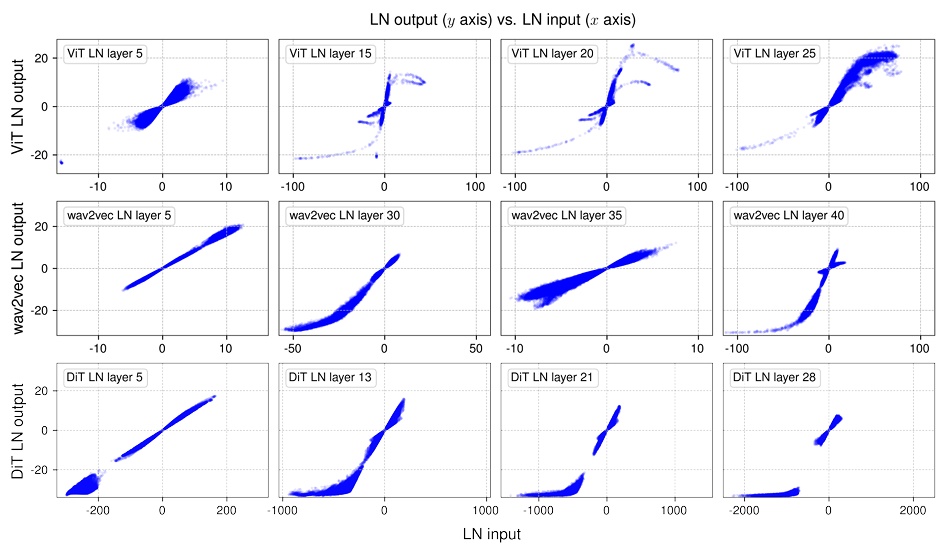
\includegraphics[width=\textwidth]{imagenes/Posibles img/LN en S.png}
        \caption{Entrada-salida producidas por LayerNorm.}
        \label{fig:ln_curva_s}
    \end{subfigure}
    \hfill
    \begin{subfigure}[b]{0.45\textwidth}
        \centering
        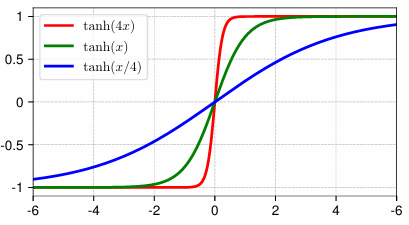
\includegraphics[width=\textwidth]{imagenes/Posibles img/Tanh.png}
        \caption{$\tanh(\alpha x)$ con tres valores diferentes de $\alpha$}
        \label{fig:tanh_alpha}
    \end{subfigure}
    \caption{Similitud entre los mapeos entrada-salida de LayerNorm y la función $\tanh$ escalada.}
    \label{fig:ln_vs_tanh}
\end{figure}
 
Para entender por qué emergen estas curvas, es útil notar que LayerNorm realiza una transformación lineal independiente para cada token. Dado el token $i$, todos sus elementos $x_{ik}$ se escalan por el mismo factor $1/\sigma_i$. Sin embargo, como cada token tiene una varianza distinta, las pendientes de estas transformaciones lineales son distintas entre sí. Cuando se visualizan en conjunto todas las activaciones del tensor, los segmentos de recta de distintas pendientes se ensamblan formando una curva en $S$ no-lineal. Las pocas activaciones con valores extremos, aquellas con $|x_{ik}|$ grande, son las más afectadas por la normalización, pues sus varianzas son altas y el factor $1/\sigma_i$ las comprime fuertemente. Este efecto de \textit{squashing} no-lineal sobre valores extremos es, según Zhu et al. (2025), la propiedad esencial de LayerNorm que explica su importancia en el entrenamiento de redes profundas.
 
Esta observación tiene una implicación directa: si el comportamiento funcional de LayerNorm es empíricamente similar al de una función $\tanh$ escalada, entonces una operación definida explícitamente como $\tanh(\alpha \mathbf{x})$ podría reproducir dicho comportamiento de manera más directa, sin necesidad de calcular estadísticas de activación.
 
\subsection{Dynamic Tanh (DyT)}
 
Inspirados por la similitud entre los mapeos de LayerNorm y la función $\tanh$, Zhu et al. (2025) \cite{Zhu2025Transformers} proponen \textit{Dynamic Tanh} (DyT) como un reemplazo directo (\textit{drop-in replacement}) de las capas de normalización en Transformers. Para un tensor de entrada $\mathbf{x}$, una capa DyT se define como:
 
\begin{equation}
\text{DyT}(\mathbf{x}) = \boldsymbol{\gamma} \cdot \tanh(\alpha \mathbf{x}) + \boldsymbol{\beta}
\end{equation}
 
donde $\alpha \in \mathbb{R}$ es un escalar aprendible que controla la escala de la entrada antes de la función $\tanh$, y $\boldsymbol{\gamma}, \boldsymbol{\beta} \in \mathbb{R}^C$ son parámetros afines aprendibles, análogos a los de LayerNorm. La operación es completamente \textit{elemento a elemento}: no requiere calcular ninguna estadística del tensor de entrada (media, varianza), lo que la distingue del resto de variantes de normalización.

\vspace{0.5cm}
\begin{figure}[htbp]
    \centering
    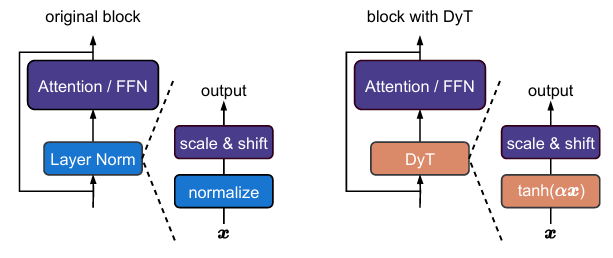
\includegraphics[width=0.5\textwidth]{imagenes/Posibles img/Posición DyT.png}
    \caption{Bloque Transformer original (Izquierda) y propuesta Transformer con DyT (Derecha). DyT reemplaza directamente a LayerNorm sin modificar el resto de la arquitectura \cite{Zhu2025Transformers}.}
    \label{fig:dyt_block}
\end{figure}
 
El parámetro $\alpha$ cumple un rol central. Al escalar la entrada antes de $\tanh$, controla la pendiente efectiva de la curva en $S$: valores grandes de $\alpha$ producen una saturación más rápida, es decir, una curva más abrupta, mientras que valores pequeños producen un comportamiento más lineal en el rango central. Durante el entrenamiento, $\alpha$ aprende a rastrear aproximadamente $1/\sigma$ de las activaciones de entrada, de manera análoga a cómo LayerNorm normaliza por la desviación estándar. Zhu et al. (2025) \cite{Zhu2025Transformers} verifican empíricamente esta correlación: los valores finales de $\alpha$ en redes entrenadas presentan una fuerte correlación positiva con $1/\sigma$ de las activaciones correspondientes.

Para entender por qué $\alpha$ converge a $1/\sigma$, es útil considerar el comportamiento de $\tanh$ en la región lineal. Para valores pequeños de $|\alpha x|$, la función $\tanh$ admite la aproximación de primer orden:

\begin{equation}
\tanh(\alpha x) \approx \alpha x, \qquad |\alpha x| \ll 1
\end{equation}

En esta región, DyT se comporta como una transformación lineal $\boldsymbol{\gamma} \cdot \alpha \mathbf{x} + \boldsymbol{\beta}$, estructuralmente análoga a la parte lineal de LayerNorm con factor de escala efectivo $\alpha$. Si la red aprende a minimizar la discrepancia entre el comportamiento de DyT y el de LayerNorm, el valor óptimo de $\alpha$ en la región central debe satisfacer $\alpha \approx 1/\sigma$, pues ese es el factor de escala que LayerNorm aplica. Fuera de la región lineal, la saturación de $\tanh$ comprime los valores extremos, replicando el efecto de \textit{squashing} de LayerNorm sobre activaciones con varianza alta. Este razonamiento conecta la observación empírica de Zhu et al. con la dinámica de optimización: $\alpha$ converge a $1/\sigma$ porque es el punto de equilibrio que minimiza la diferencia funcional entre DyT y LayerNorm para las activaciones de la red. A diferencia de LayerNorm, donde el factor de escala $1/\sigma$ se recalcula explícitamente en cada pasada hacia adelante a partir de las estadísticas del batch, en DyT este factor emerge de manera implícita como consecuencia del entrenamiento: la red aprende a normalizarse a sí misma sin requerir cómputo de estadísticas, lo que constituye una forma de normalización paramétrica en contraste con la normalización estadística de LayerNorm.

\vspace{0.5cm}
\begin{figure}[htbp]
    \centering
    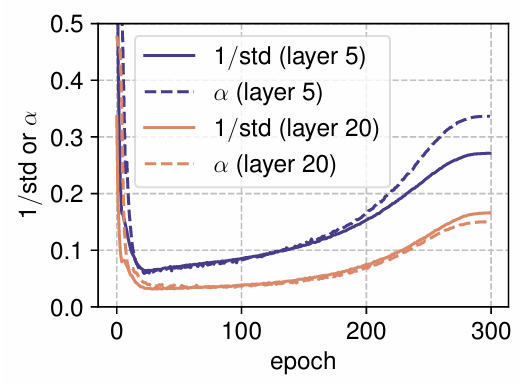
\includegraphics[width=0.4\textwidth]{imagenes/Posibles img/Sigma vs alpha.png}
    \caption{Seguimiento de $1/\sigma$ y $\alpha$ a final de cada época.}
    \label{fig:sigma_vs_alpha}
\end{figure}
 
La inicialización de $\alpha$ es relevante para la estabilidad del entrenamiento. Para modelos no-LLM, Zhu et al. (2025) \cite{Zhu2025Transformers} recomiendan $\alpha_0 = 0{.}5$ como valor por defecto, con $\boldsymbol{\gamma}$ inicializado en $\mathbf{1}$ y $\boldsymbol{\beta}$ en $\mathbf{0}$, en analogía directa con la inicialización estándar de LayerNorm. Con esta configuración, DyT produce curvas de convergencia prácticamente idénticas a las de LN sin necesidad de ajustar ningún otro hiperparámetro del modelo original.
 
\subsection{LayerNorm vs DyT}
 
La diferencia estructural más importante entre LayerNorm y DyT es la ausencia de cálculo de estadísticas en DyT. En LayerNorm, cada pasada hacia adelante requiere calcular $\mu$ y $\sigma^2$ sobre las $C$ dimensiones de cada token, lo que implica una operación de reducción (\textit{reduction}) que introduce dependencias entre elementos del tensor. DyT, al ser completamente elemento a elemento, elimina esta dependencia.
 
Las diferencias funcionales más sustanciales son las siguientes. LayerNorm normaliza \textit{por token}: cada token es escalado por su propia desviación estándar, lo que hace que la transformación sea adaptativa a las estadísticas locales de cada posición temporal. DyT, en cambio, aplica un único escalar global $\alpha$ a todas las posiciones, lo que equivale a una normalización colectiva del tensor completo. Esta distinción es relevante para series temporales con alta variabilidad entre pasos: LayerNorm se adapta localmente a cada paso, mientras que DyT aprende un comportamiento promedio. La segunda diferencia relevante es que LayerNorm centra las activaciones (resta la media), mientras que DyT no lo hace explícitamente. La función $\tanh$ es impar y centrada en cero, lo que introduce un sesgo implícito hacia el centrado, pero sin la garantía de media exactamente cero que provee LayerNorm.

Un aspecto adicional relevante es la elección de la función de \textit{squashing}. Zhu et al. (2025) evalúan alternativas a $\tanh$ en DyT: la función identidad (sin squashing), \textit{hardtanh} y sigmoide. 

\vspace{0.5cm}
\begin{figure}[htbp]
    \centering
    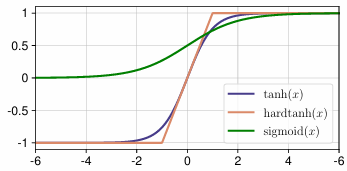
\includegraphics[width=0.4\textwidth]{imagenes/Posibles img/Tanh Hard Sigmoid.png}
    \caption{Curvas de tres funciones squashing: tanh, hardtanh y sigmoide.}
    \label{fig:squashing_functions}
\end{figure}

Los resultados muestran que la ausencia de squashing produce divergencia del entrenamiento, lo que confirma que el efecto de compresión de valores extremos es indispensable. Entre las funciones de squashing, $\tanh$ supera a las demás en rendimiento, lo que los autores atribuyen a dos propiedades: su \textit{suavidad} (es infinitamente diferenciable, a diferencia de \textit{hardtanh} que tiene discontinuidades en la derivada) y su \textit{simetría} respecto al cero (es una función impar, lo que favorece gradientes equilibrados durante el entrenamiento). Estas propiedades hacen que $\tanh$ sea la función de squashing más apta para reemplazar LayerNorm en Transformers.

\vspace{0.5cm}
\begin{figure}[htbp]
    \centering
    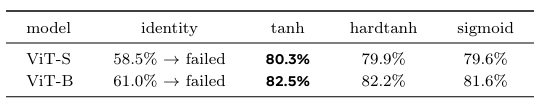
\includegraphics[width=0.5\textwidth]{imagenes/Posibles img/Resultados sigmoid.png}
    \caption{Accuracy de clasificación en ImageNet-1K con diferentes funciones de squashing}
    \label{fig:resultados_squashing_functions}
\end{figure}
 
En términos de rendimiento empírico, Zhu et al. (2025) reportan que DyT iguala o supera a LayerNorm en una amplia variedad de tareas y arquitecturas: clasificación de imágenes, aprendizaje auto-supervisado, modelos de difusión, modelos de lenguaje LLaMA (7B a 70B), habla y secuencias genómicas, entrenados con los mismos hiperparámetros del modelo original con LayerNorm y sin ajuste adicional, lo que respalda su uso como reemplazo directo también en el TFT de este trabajo.

\subsection{Uso de DyT en el TFT para predicción de costos marginales}
 
En el modelo propuesto en este trabajo, DyT reemplaza a LayerNorm en todos los puntos donde esta aparece en la arquitectura TFT: dentro de cada bloque GRN (en la conexión residual final), en las conexiones residuales con compuerta (\textit{gated skip connections}) de la capa LSTM, en la capa de enriquecimiento estático y en la capa de auto-atención interpretable. La sustitución es uniforme y directa: cada ocurrencia de $\text{LayerNorm}(\mathbf{a} + \text{GLU}(\cdot))$ en las ecuaciones de la Sección 2.3.4 se reemplaza por $\text{DyT}(\mathbf{a} + \text{GLU}(\cdot))$, manteniendo inalterada la estructura del bloque.

El parámetro $\alpha$ es independiente para cada capa DyT de la red, lo que significa que el TFT aprende factores de escala distintos para cada GRN, cada conexión residual del LSTM y cada capa de atención. Esta flexibilidad permite que la red calibre el grado de squashing de manera diferenciada según la variabilidad de las activaciones en cada módulo.
 
La motivación principal para adoptar DyT en este contexto es la naturaleza de las series de costo marginal en el Sistema Eléctrico Nacional (SEN). Los costos marginales horarios presentan una distribución fuertemente asimétrica con colas pesadas: en condiciones normales los valores se ubican en el rango de \$20 a \$80 USD/MWh, pero durante eventos de escasez hídrica, fallas de generación o congestiones de transmisión pueden producirse \textit{spikes} que superan los \$300 USD/MWh, valores que exceden en más de un orden de magnitud el rango habitual. En el contexto de la arquitectura TFT, estos valores extremos se propagan como activaciones de gran magnitud a través de los bloques GRN y las capas de atención. LayerNorm los comprime normalizando por la desviación estándar del token correspondiente, pero esta compresión depende de la estadística local de cada paso temporal, lo que puede generar gradientes inestables cuando un token aislado contiene un valor extremo rodeado de valores normales. DyT, al aplicar la saturación de $\tanh$ directamente sobre las activaciones mediante el escalar global $\alpha$, comprime los valores extremos de manera más uniforme e independiente de la estadística local, actuando como una forma de regularización implícita sobre los spikes del costo marginal.

Una segunda consideración es la interacción entre DyT y el mecanismo de atención interpretable del TFT. Dado que los pesos de atención $\tilde{\mathbf{A}}_{ij}$ se calculan sobre representaciones que ya han pasado por la capa de enriquecimiento estático con DyT, la compresión de activaciones extremas garantiza que los scores de atención no sean dominados por spikes temporales, lo que favorece la interpretabilidad: los instantes pasados más relevantes para la predicción reflejan patrones estructurales del mercado eléctrico y no artefactos de valores atípicos.
 
La inicialización de $\alpha$ sigue la recomendación de Zhu et al. (2025) para modelos no-LLM, fijando $\alpha_0 = 0{.}5$ con $\boldsymbol{\gamma} = \mathbf{1}$ y $\boldsymbol{\beta} = \mathbf{0}$. Con esta configuración, el TFT con DyT puede entrenarse directamente con los mismos hiperparámetros utilizados en la versión con LayerNorm, sin requerir ajuste adicional, lo que simplifica el proceso de búsqueda de hiperparámetros y hace la comparación entre ambas versiones directamente interpretable.

En el contexto del modelo híbrido propuesto, la elección de DyT tiene una implicancia adicional que va más allá del rendimiento individual del TFT. Dado que el esquema de Stacking Optimization descrito en la Sección 2.5 combina las predicciones del TFT con LayerNorm, el TFT con DyT y Prophet mediante una combinación lineal con pesos aprendidos, la diversidad entre los modelos base es un factor determinante de la calidad del ensamblaje: modelos que cometen errores distintos y poco correlacionados se complementan mejor que modelos similares. Al reemplazar LayerNorm por DyT se introduce una diferencia estructural en el mecanismo de normalización que, en presencia de spikes del costo marginal, puede producir distribuciones de error cualitativamente distintas entre ambas variantes del TFT. Esta diversidad estructural es precisamente lo que el Stacking Optimization puede explotar para mejorar la predicción conjunta, haciendo de la comparación LayerNorm versus DyT no solo un experimento de ablación sino un componente funcional del modelo híbrido.

\section{Stacking Optimization}

El \textit{Stacking}, también denominado \textit{stacked generalization}, es una técnica de ensamblaje de modelos introducida por Wolpert (1992) \cite{StackingWolpert} que combina las predicciones de múltiples modelos base mediante un metamodelo entrenado para minimizar el error de predicción conjunta. A diferencia de métodos de ensamblaje más simples como el promedio o el voto mayoritario, el Stacking aprende los pesos de combinación de forma supervisada, lo que le permite asignar mayor importancia a los modelos base que presentan menor error en las regiones del espacio de entrada donde los demás fallan.

La intuición central del Stacking es la siguiente: distintos modelos base capturan aspectos complementarios de la distribución de los datos, y el metamodelo puede explotar esta complementariedad combinando sus predicciones de manera que se cancelen los errores individuales. Para que esta cancelación sea efectiva, es necesario que los errores de los modelos base estén escasamente correlacionados, condición que se denomina \textit{diversidad del ensamble} \cite{Dietterich}.

\subsection{Formulación general y diversidad del ensamble}

Sea $\{M_k\}_{k=1}^K$ un conjunto de $K$ modelos base, donde cada modelo $M_k$ produce una predicción $\hat{y}_t^{(k)}$ para el instante $t$, concatenadas en el vector de meta-características $\tilde{\mathbf{z}}_t = (\hat{y}_t^{(1)}, \ldots, \hat{y}_t^{(K)})^\top \in \mathbb{R}^K$. El Stacking, en la forma lineal empleada en este trabajo, combina estas predicciones con pesos $\boldsymbol{\alpha} = (\alpha_1, \ldots, \alpha_K)^\top$:

\begin{equation}
    \hat{y}_t^{\text{stack}} = \sum_{k=1}^{K} \alpha_k\, \hat{y}_t^{(k)} = \boldsymbol{\alpha}^\top \tilde{\mathbf{z}}_t
    \label{eq:stacking_lineal}
\end{equation}

estimados minimizando el error cuadrático medio sobre un conjunto de validación:

\begin{equation}
    \hat{\boldsymbol{\alpha}} = \operatorname*{arg\,min}_{\boldsymbol{\alpha}} \sum_{t \in \mathcal{V}} \left(y_t - \boldsymbol{\alpha}^\top \tilde{\mathbf{z}}_t\right)^2
    \label{eq:stacking_opt}
\end{equation}

donde $\mathcal{V}$ denota el conjunto de índices de validación; en la práctica esta minimización se resuelve mediante métodos analíticos (mínimos cuadrados) o metaheurísticos (Sección 3.5.2).

La ganancia teórica del Stacking sobre cualquiera de los modelos base individuales depende de la diversidad de los errores de predicción. Si $\varepsilon_t^{(k)} = y_t - \hat{y}_t^{(k)}$ denota el error del modelo $k$ en el instante $t$, el error del ensamble es $\varepsilon_t^{\text{stack}} = \sum_{k=1}^K \alpha_k\, \varepsilon_t^{(k)}$ y, asumiendo $\sum_k \alpha_k = 1$, su varianza es:

\begin{equation}
    \text{Var}\!\left(\varepsilon_t^{\text{stack}}\right) = \boldsymbol{\alpha}^\top \boldsymbol{\Sigma}\, \boldsymbol{\alpha}
\end{equation}

donde $\boldsymbol{\Sigma} \in \mathbb{R}^{K \times K}$ es la matriz de covarianzas de los errores, con $\Sigma_{ij} = \text{Cov}(\varepsilon_t^{(i)}, \varepsilon_t^{(j)})$: esta varianza solo se reduce por debajo de la de los modelos base individuales cuando sus errores están poco correlacionados, y no se reduce en absoluto si están perfectamente correlacionados \cite{Dietterich}. Esta observación justifica la importancia de seleccionar modelos base estructuralmente distintos. Cuando los modelos base presentan predicciones muy correlacionadas, la matriz de diseño $\tilde{\mathbf{Z}} = (\tilde{\mathbf{z}}_t)_{t \in \mathcal{V}}$ puede ser casi singular, lo que hace preferible la estimación regularizada mediante regresión de Ridge:

\begin{equation}
    \hat{\boldsymbol{\alpha}} = \left(\tilde{\mathbf{Z}}^\top \tilde{\mathbf{Z}} + \lambda \mathbf{I}\right)^{-1} \tilde{\mathbf{Z}}^\top \mathbf{y}_\mathcal{V}
    \label{eq:stacking_ridge}
\end{equation}

donde $\lambda > 0$ es el parámetro de regularización y $\mathbf{y}_\mathcal{V}$ es el vector de valores observados en el conjunto de validación.

\subsection{Protocolo de entrenamiento y prevención de data leakage}

Un aspecto crítico del Stacking en el contexto de series temporales es la prevención del \textit{data leakage} al construir el conjunto de meta-características. En problemas de clasificación o regresión con datos i.i.d., el procedimiento estándar consiste en generar las predicciones de los modelos base mediante validación cruzada $k$-fold: cada modelo base se entrena en los $k-1$ folds restantes y produce predicciones fuera de muestra para el fold reservado, de modo que las meta-características $\tilde{\mathbf{z}}_t$ son siempre predicciones fuera de muestra \cite{StackingWolpert}. Este protocolo garantiza que el metamodelo se entrena sobre predicciones que no han visto los datos de entrenamiento de los modelos base, evitando sobreajuste.

En series temporales, la validación cruzada estándar no es aplicable porque viola el orden temporal de las observaciones: entrenar con datos futuros para predecir el pasado inflaría artificialmente el rendimiento de los modelos base y produciría meta-características con filtración de información. El protocolo correcto para series temporales es la \textit{validación cruzada con expansión temporal} (\textit{time series split}), ilustrada en la Figura \ref{fig:tss}:

\begin{enumerate}
    \item Se divide la serie en $K+1$ bloques cronológicos de igual tamaño.
    \item En la iteración $k \in \{1, \ldots, K\}$, los modelos base se entrenan sobre los primeros $k$ bloques y producen predicciones fuera de muestra sobre el bloque $k+1$.
    \item Las predicciones fuera de muestra de todos los modelos base para cada observación se concatenan para formar $\tilde{\mathbf{z}}_t$.
    \item El metamodelo se entrena sobre $\{\tilde{\mathbf{z}}_t, y_t\}_{t \in \mathcal{V}}$, donde $\mathcal{V}$ es el conjunto de validación final, cronológicamente posterior al período de entrenamiento de los modelos base.
\end{enumerate}

Este protocolo garantiza que en ningún punto se utilizan observaciones futuras para generar las meta-características, preservando la causalidad temporal del proceso de estimación.

\vspace{0.5cm}
\begin{figure}[htbp]
    \centering
    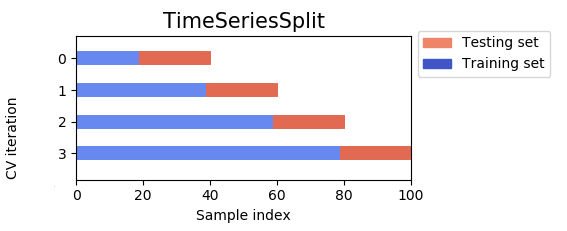
\includegraphics[width=0.5\textwidth]{imagenes/Posibles img/Time Series Split.png}
    \caption{Visualización de Time Series Split.}
    \label{fig:tss}
\end{figure}

El procedimiento de $K$ iteraciones descrito arriba resuelve un problema específico: cuando los modelos base deben reentrenarse en cada fold para que sus predicciones sobre ese fold sean genuinamente fuera de muestra, un único split no basta, porque el conjunto usado para ajustar cada modelo base cambiaría de tamaño y período de un fold a otro si no se repite el ajuste. En el modelo híbrido de este trabajo (Sección 2.5.3), en cambio, cada modelo base --Prophet, $\text{TFT}_\text{LN}$ y $\text{TFT}_\text{DyT}$-- se ajusta una única vez sobre el conjunto de entrenamiento (Sección 3.2), y sus predicciones sobre el conjunto de validación son, por construcción, siempre fuera de muestra: ninguna observación de validación participa del ajuste de ningún modelo base, sin necesidad de repetir el ajuste en múltiples folds para lograrlo. El Stacking Optimization aplicado en este trabajo (Sección 3.5.1) usa, por lo tanto, un único split cronológico train/validación/prueba en lugar de la validación cruzada con expansión temporal de $K$ iteraciones: ambos esquemas evitan la misma fuga de información --que el metamodelo vea predicciones de un modelo base sobre datos que ese modelo ya usó para entrenarse--, pero el split único es suficiente aquí porque esa condición ya se cumple sin necesidad de reajustar los modelos base repetidamente, y evita el costo computacional adicional de entrenar cada modelo base $K$ veces.

\subsection{Stacking Optimization en el modelo híbrido propuesto}

El modelo propuesto en este trabajo dispone de tres predicciones puntuales por barra: Prophet, el TFT con LayerNorm entrenado sobre los residuos de Prophet (denominado $\text{TFT}_\text{LN}$, en su versión de residuos o de precios directos) y el TFT con DyT sobre la serie original (denominado $\text{TFT}_\text{DyT}$). En vez de resolver un único problema de $K=3$ pesos simultáneos como en la formulación general de \eqref{eq:stacking_opt}, el Stacking Optimization aplicado en este trabajo evalúa, para cada barra y cada arquitectura (LN y DyT, por separado), varias combinaciones \textbf{de a lo más dos componentes} a la vez:

\begin{equation}
    \hat{y}_t^{(b),\,\text{Stack}} = w_1^{(b)}\,\hat{y}_t^{(b),\,(1)} + w_2^{(b)}\,\hat{y}_t^{(b),\,(2)}, \qquad w_1^{(b)} + w_2^{(b)} = 1,\;\; w_1^{(b)}, w_2^{(b)} \geq 0
    \label{eq:stacking_hibrido}
\end{equation}

donde el par $\big(\hat{y}^{(1)}, \hat{y}^{(2)}\big)$ instancia una de varias estrategias candidatas --desde un modelo base solo, sin combinar, hasta la combinación de Prophet con la predicción de precios o de residuos del TFT correspondiente-- detalladas junto con sus pesos fijos u optimizados en la Sección 3.5.1. La restricción a dos componentes por combinación, en lugar de una única combinación simultánea de los tres, permite aislar qué par de modelos aporta la mejor combinación por barra, en vez de forzar una única estructura de ensamble para las ocho barras del SEN. Los pesos $(w_1^{(b)}, w_2^{(b)})$ de cada estrategia se estiman por separado para cada barra, minimizando el \textbf{MAE} sobre el conjunto de validación --no el objetivo de mínimos cuadrados de \eqref{eq:stacking_opt}--, dado que el MAE es la métrica de referencia del resto de este trabajo y es más robusto a los \textit{outliers} de cola pesada del costo marginal que el error cuadrático. Al no admitir una solución cerrada como \eqref{eq:stacking_ridge}, la optimización se resuelve con métodos numéricos (búsqueda en grilla, optimización directa, búsqueda aleatoria), descritos junto con la regularización Ridge --incluida como una de las alternativas comparadas, no como el método adoptado-- en la Sección 3.5.2.

La motivación para incluir los tres modelos base como candidatos responde directamente al principio de diversidad discutido en la Sección 2.5.1. Prophet captura la estructura de largo plazo de la serie mediante descomposición aditiva interpretable, pero sus errores son sistemáticos en presencia de fluctuaciones no lineales de corto plazo. El $\text{TFT}_\text{LN}$ modela la variabilidad residual de corto plazo y hereda la estabilidad de LayerNorm frente a secuencias de amplitud moderada. El $\text{TFT}_\text{DyT}$, al operar sobre la serie completa con la compresión de $\tanh$, es más robusto frente a los \textit{spikes} del costo marginal descritos en la Sección 2.4.4, pero puede sobreajustar la tendencia en períodos de baja volatilidad. Esta heterogeneidad estructural en los patrones de error favorece covarianzas $\text{Cov}(\varepsilon^{(i)}, \varepsilon^{(j)})$ pequeñas en magnitud entre cualquier par de modelos base, lo que, por la descomposición de la varianza del ensamble de \eqref{eq:stacking_opt}, respalda que combinar dos de ellos pueda producir ganancias de predicción medibles respecto a cualquiera por separado.

Finalmente, la predicción puntual $\hat{y}_t^{(b),\,\text{Stack}}$ de la mejor estrategia por barra sirve como centro de los intervalos de predicción construidos mediante Conformal Prediction en la Sección 2.6.

\section{Conformal Prediction}

La \textit{Predicción Conforme} o \textit{Conformal Prediction} (CP) es un marco estadístico para construir intervalos de predicción con garantías de cobertura finita sin supuestos distribucionales sobre los datos, más allá de la intercambiabilidad \cite{VovkCP}. A diferencia de los métodos probabilísticos clásicos, cuyas garantías son asintóticas o requieren supuestos paramétricos sobre el modelo, CP produce intervalos válidos para cualquier algoritmo de predicción subyacente, incluyendo redes neuronales, modelos de ensamble y modelos híbridos como el propuesto en este trabajo.

Formalmente, dado un nivel de no-cobertura $\alpha \in (0,1)$ fijado por el usuario, el objetivo es construir un intervalo de predicción $C_{n,\alpha}(x_{n+1})$ tal que:

\begin{equation}
    \mathbb{P}\!\left\{Y_{n+1} \in C_{n,\alpha}(X_{n+1})\right\} \geq 1 - \alpha
    \label{eq:cp_coverage}
\end{equation}

Un intervalo que satisface \eqref{eq:cp_coverage} se denomina \textit{marginalmente válido}. Al mismo tiempo, se exige que el intervalo sea \textit{eficiente}, es decir, lo más estrecho posible: intervalos excesivamente anchos son válidos pero no informativos. El equilibrio entre validez y eficiencia es el criterio central para comparar las distintas variantes de CP \cite{ConformalPrediction}.

La propiedad de intercambiabilidad es el supuesto base de CP: una secuencia aleatoria $(Z_1, \ldots, Z_n)$ es intercambiable si su distribución conjunta es invariante bajo cualquier permutación de los índices. Este supuesto es más débil que la independencia e idéntica distribución (i.i.d.), pero excluye las series temporales, donde la dependencia temporal viola la intercambiabilidad. Esta limitación motiva las variantes adaptativas de CP descritas en las siguientes Secciones.

\subsection{Split Conformal Prediction (SCP)}

La \textit{Split Conformal Prediction} (SCP) es la variante más simple y computacionalmente eficiente de CP, introducida por Papadopoulos et al. (2002) y reformulada por Lei et al. (2018) \cite{LeiCP}. Su idea central es dividir el conjunto de entrenamiento en dos partes: un subconjunto de entrenamiento propio $\mathcal{T}r$ y un conjunto de calibración $\mathcal{C}al$, de modo que el modelo se ajusta solo sobre $\mathcal{T}r$ y los residuos sobre $\mathcal{C}al$ se usan para construir el intervalo.

Dado un modelo de predicción $\hat{\mu}$ ajustado sobre $\mathcal{T}r$, se define la \textit{puntuación de conformidad} (\textit{conformity score}) de cada punto de calibración como el residuo absoluto:

\begin{equation}
    S_i = \left|y_i - \hat{\mu}(x_i)\right|, \quad i \in \mathcal{C}al
    \label{eq:conformity_score}
\end{equation}

El conjunto de puntuaciones de calibración es $\mathcal{S} = \{S_i\}_{i \in \mathcal{C}al} \cup \{+\infty\}$, donde el valor $+\infty$ se añade para garantizar la validez de cobertura en muestra finita. Se calcula el cuantil corregido de nivel $1 - \alpha$ sobre $\mathcal{S}$:

\begin{equation}
    \hat{q}_{1-\alpha}(\mathcal{S}) = \text{Cuantil}\!\left(1 - \alpha;\, \mathcal{S}\right)
    \label{eq:quantile_scp}
\end{equation}

El intervalo de predicción para un nuevo punto $x_{n+1}$ es entonces:

\begin{equation}
    C_{n,\alpha}(x_{n+1}) = \left[\hat{\mu}(x_{n+1}) - \hat{q}_{1-\alpha}(\mathcal{S}),\; \hat{\mu}(x_{n+1}) + \hat{q}_{1-\alpha}(\mathcal{S})\right]
    \label{eq:scp_interval}
\end{equation}

\begin{teorema}[Validez marginal de SCP \cite{LeiCP}]

Si $(X_1, Y_1), \ldots, (X_n, Y_n), (X_{n+1}, Y_{n+1})$ son intercambiables y $\hat{\mu}$ es independiente del conjunto de calibración $\mathcal{C}al$, entonces el intervalo \eqref{eq:scp_interval} satisface:

\begin{equation}
    1 - \alpha \;\leq\; \mathbb{P}\!\left\{Y_{n+1} \in C_{n,\alpha}(X_{n+1})\right\} \;\leq\; 1 - \alpha + \frac{1}{|\mathcal{C}al| + 1}
    \label{eq:scp_validity}
\end{equation}
\end{teorema}

La cota superior en \eqref{eq:scp_validity} muestra que la cobertura excede el nivel nominal en a lo más $\frac{1}{|\mathcal{C}al|+1}$, un término que tiende a cero conforme crece el conjunto de calibración. En la práctica, mantener entre el 10\% y el 30\% del conjunto de entrenamiento para calibración es un compromiso adecuado entre el tamaño del conjunto de calibración y la precisión del modelo ajustado \cite{ConformalPrediction}.

La principal limitación de SCP es que produce intervalos de ancho constante, independiente de las covariables $x_{n+1}$: el cuantil $\hat{q}_{1-\alpha}(\mathcal{S})$ es un escalar global, lo que implica que el intervalo tendrá el mismo ancho para instantes con alta volatilidad que para instantes con precios estables. En el contexto del SEN, donde los spikes del costo marginal concentran la incertidumbre en regímenes específicos, esta rigidez reduce la eficiencia del intervalo. La segunda limitación, más fundamental para series temporales, es que la garantía \eqref{eq:scp_validity} requiere intercambiabilidad, supuesto que no se cumple en datos con dependencia temporal.

\subsection{Regresión Cuantílica Conformada (CQR)}

La \textit{Conformalized Quantile Regression} (CQR), propuesta por Romano et al. (2019) \cite{RomanoCQR}, aborda la limitación de ancho constante de SCP reemplazando el predictor puntual $\hat{\mu}$ por un par de modelos de regresión cuantílica, $\hat{q}_{\alpha/2}$ y $\hat{q}_{1-\alpha/2}$, ajustados de modo que el intervalo se adapte a la covariable $x$ desde el propio modelo base, sin requerir una estimación de escala externa.

Sobre el conjunto de calibración $\mathcal{C}al$, el \textit{score} de conformidad se define como la mayor violación observada de cualquiera de los dos cuantiles:

\begin{equation}
    S_i = \max\left\{\hat{q}_{\alpha/2}(x_i) - y_i,\; y_i - \hat{q}_{1-\alpha/2}(x_i)\right\}, \quad i \in \mathcal{C}al
    \label{eq:cqr_score}
\end{equation}

Un valor positivo de $S_i$ indica que el intervalo cuantílico no cubrió la observación $i$ (por abajo o por arriba); uno negativo indica que la cubrió con margen. El cuantil corregido $\hat{q}_{1-\alpha}(\mathcal{S})$ se calcula sobre estos scores con la misma corrección de muestra finita de \eqref{eq:quantile_scp}, y el intervalo final para un nuevo punto $x_{n+1}$ se obtiene expandiendo los cuantiles estimados en ese margen constante:

\begin{equation}
    C_{n,\alpha}(x_{n+1}) = \left[\hat{q}_{\alpha/2}(x_{n+1}) - \hat{q}_{1-\alpha}(\mathcal{S}),\; \hat{q}_{1-\alpha/2}(x_{n+1}) + \hat{q}_{1-\alpha}(\mathcal{S})\right]
    \label{eq:cqr_interval}
\end{equation}

A diferencia de SCP, donde el ancho del intervalo es un escalar fijo, en CQR el ancho $\hat{q}_{1-\alpha/2}(x) - \hat{q}_{\alpha/2}(x)$ varía con $x$ porque proviene directamente de los modelos cuantílicos; el término $\hat{q}_{1-\alpha}(\mathcal{S})$ solo corrige el sesgo de cobertura de esos cuantiles, preservando la garantía de validez marginal \eqref{eq:scp_validity} bajo el mismo supuesto de intercambiabilidad.

En la implementación utilizada en este trabajo, los modelos de regresión cuantílica son lineales con penalización $\ell_1$ y se ajustan sobre tres variables: la predicción puntual del TFT, $\hat{y}_t$, y las componentes seno y coseno de la hora del día, $\sin(2\pi h_t/24)$ y $\cos(2\pi h_t/24)$, de modo que CQR también incorpora, de forma paramétrica y continua, la heterocedasticidad horaria que motiva a LW Split CP y LW-ACP (Sección \ref{sec:lwacp}). La calibración se realiza mediante validación cruzada de $K$ pliegues sobre el conjunto de validación, sin mezclar el orden temporal (\textit{K-fold cross-conformal}), acumulando los scores de calibración de todos los pliegues antes de calcular $\hat{q}_{1-\alpha}(\mathcal{S})$, lo que evita la inestabilidad observada al calibrar sobre un único split temporal fijo. CQR se emplea en este trabajo como método de comparación externo a la familia de Conformal Prediction, evaluado, al igual que Split CP, ACI y las variantes ponderadas localmente (Sección \ref{sec:lwacp}), sobre las ocho barras del pipeline S+C descrito en el Capítulo 3.

\subsection{Conformal Prediction con Ensemble (EnbPI)}

\textit{Ensemble Prediction Interval} o \textit{EnbPI}, fue propuesto por Xu y Xie (2021) \cite{XuCP} como una adaptación de CP a series temporales mediante \textit{bootstrap} de un ensamble de modelos, cuyos residuos \textit{leave-one-out} se acumulan en una ventana deslizante de \textit{scores} de calibración que se actualiza secuencialmente sin reajustar el modelo subyacente. Xu y Xie (2021) proponen además la variante \textit{EnbPI V2} \cite{ConformalPrediction}, que agrega por media en todas las fases del procedimiento en lugar de mezclar media y cuantil, mejorando la cobertura empírica. Este trabajo no implementa EnbPI: su mecanismo de \textit{bootstrap} está diseñado para un modelo base entrenable con múltiples réplicas, mientras que S+C-LN, la estrategia de referencia adoptada (Sección 4.4.5), es una única predicción del TFT sin ensamble subyacente que bootstrapear.

\subsection{Adaptive Conformal Inference (ACI)}

La \textit{Adaptive Conformal Inference} (ACI) fue propuesta por Gibbs y Candès (2021) \cite{GibbsCP} para adaptarse a series temporales bajo cambios de distribución arbitrarios. La idea central de ACI es reemplazar el nivel de no-cobertura fijo $\alpha$ por un nivel efectivo $\alpha_t$ que se actualiza recursivamente en función del historial de cobertura:

\begin{equation}
    \alpha_{t+1} = \alpha_t + \gamma\left(\alpha - \mathbf{1}\!\left\{y_t \notin C_t(x_t)\right\}\right)
    \label{eq:aci_update}
\end{equation}

donde $\gamma > 0$ es un hiperparámetro de tasa de aprendizaje y $\mathbf{1}\{\cdot\}$ es la función indicadora. La lógica de la actualización \eqref{eq:aci_update} es la siguiente: si en el instante $t$ el intervalo no cubre el valor real ($y_t \notin C_t$), entonces $\alpha_{t+1} < \alpha_t$, lo que amplía el intervalo en la siguiente predicción; si cubre, $\alpha_{t+1} > \alpha_t$, reduciendo el intervalo. Inicialmente se fija $\alpha_1 = \alpha$.

El intervalo de predicción en el instante $t$ se construye con el nivel actualizado:

\begin{equation}
    C_t(x_t) = \left[\hat{\mu}_t(x_t) - \hat{q}_{1-\alpha_t}(\mathcal{S}_{\mathcal{C}al_t}),\; \hat{\mu}_t(x_t) + \hat{q}_{1-\alpha_t}(\mathcal{S}_{\mathcal{C}al_t})\right]
    \label{eq:aci_interval}
\end{equation}

donde $\hat{\mu}_t$ es el modelo reajustado en el instante $t$ sobre los $T_0$ puntos más recientes y $\mathcal{S}_{\mathcal{C}al_t}$ es el conjunto de scores del conjunto de calibración en el instante $t$.

La garantía de cobertura de ACI es asintótica: bajo cualquier distribución de los datos, la frecuencia de no-cobertura converge al nivel nominal \cite{GibbsCP}:

\begin{equation}
    \frac{1}{T_1}\sum_{t=T_0+1}^{T_0+T_1} \mathbf{1}\!\left\{y_t \notin C_t(x_t)\right\} \xrightarrow{a.s.} \alpha, \quad T_1 \to \infty
    \label{eq:aci_asymptotic}
\end{equation}

El parámetro $\gamma$ tiene un impacto crítico sobre la eficiencia de ACI. Zaffran et al. (2022) \cite{ZaffranICML2022} demuestran que en el caso intercambiable, la longitud esperada del intervalo crece linealmente con $\gamma$, mientras que en series con dependencia temporal de tipo AR(1), existe un $\gamma^* > 0$ que minimiza la longitud esperada. Este resultado ilustra el compromiso fundamental de ACI: un $\gamma$ pequeño produce intervalos eficientes cuando los datos son casi intercambiables, pero pierde cobertura cuando la dependencia temporal es fuerte; un $\gamma$ grande garantiza cobertura incluso bajo alta dependencia, pero a costa de generar intervalos ocasionalmente infinitos.

Este compromiso motiva a AgACI (\textit{Aggregated Adaptive Conformal Inference}, Zaffran et al., 2022 \cite{ZaffranICML2022}), una extensión de ACI que evita fijar un único $\gamma$ de antemano: en cada paso, AgACI entrena en paralelo un conjunto de instancias de ACI con distintos valores de $\gamma$ y agrega sus intervalos mediante un esquema de expertos \textit{online} (\textit{Bernstein Online Aggregation}) que pondera cada instancia según su desempeño reciente, heredando garantías de regret acotado de la literatura de agregación de expertos. Es, en ese sentido, el sucesor directo de ACI para el problema específico que este trabajo aborda al fijar $\gamma = 0.05$ de antemano (Sección \ref{sec:aci_metodologia}). Este trabajo no lo implementa por alcance: agregar $\gamma$ mediante expertos introduce un mecanismo adicional (la propia agregación) cuya interacción con la ponderación horaria de LW-ACP no está caracterizada en la literatura, y evaluarla de forma rigurosa, no solo como una variante más, excede el tiempo disponible; queda como comparación externa natural para trabajo futuro, señalada explícitamente aquí en vez de omitirse.

En su formulación original, ACI reajusta el modelo de predicción puntual $\hat{\mu}_t$ en cada instante $t$ sobre una ventana deslizante de observaciones recientes, lo que permite adaptarse a cambios de distribución en el modelo base y no solo en el nivel de cobertura. En este trabajo, en cambio, $\hat{\mu}_t$ es siempre la predicción puntual ya calculada de S+C-LN, fija durante todo el período de prueba: no se reajusta ningún modelo en cada paso, ni el de predicción puntual ni el conjunto de calibración, y el único componente que evoluciona en el tiempo es el nivel $\alpha_t$ (Sección \ref{sec:aci_metodologia}). Esta simplificación, que evita el costo computacional de reentrenar en cada paso, es posible porque S+C-LN no requiere un meta-modelo reentrenable como predictor puntual, a diferencia de formulaciones de ACI sobre un ensamble.

\subsection{CP ponderado localmente: LW Split CP y LW-ACP}
\label{sec:lwacp}

Todas las variantes anteriores comparten una limitación: el cuantil de no conformidad $q$ se calcula sobre un único conjunto de \textit{scores} de calibración, tratando la incertidumbre del modelo como homogénea a lo largo de todo el horizonte de predicción. En el SEN, sin embargo, el error del modelo no es homocedástico en el tiempo: la volatilidad del costo marginal se concentra sistemáticamente en las horas de transición solar (entrada y salida del bloque fotovoltaico), mientras que las horas de mediodía, con generación solar estable, presentan errores sustancialmente menores. Un intervalo de ancho fijo o adaptado únicamente al historial global de errores está necesariamente mal calibrado en algún subconjunto de horas: demasiado ancho cuando la volatilidad es baja, demasiado angosto cuando es alta.

Esta observación motiva la construcción de \textit{scores} de no conformidad \textit{normalizados}, una técnica clásica en la literatura de CP para producir intervalos adaptados a la heterocedasticidad de los datos \cite{VovkCP}. En lugar de calibrar directamente sobre el residuo absoluto $s_t = |y_t - \hat{y}_t|$, se normaliza cada score por una estimación local de la escala del error, $\hat{\sigma}(x_t)$, específica del contexto del punto $t$:

\begin{equation}
    \tilde{s}_t = \frac{|y_t - \hat{y}_t|}{\hat{\sigma}(x_t)}
    \label{eq:lw_score}
\end{equation}

El intervalo resultante, $C_t = [\hat{y}_t - q \cdot \hat{\sigma}(x_t),\; \hat{y}_t + q \cdot \hat{\sigma}(x_t)]$, con $q$ el cuantil de los scores normalizados $\{\tilde{s}_i\}$, se ensancha o contrae proporcionalmente a $\hat{\sigma}(x_t)$, en lugar de mantener un ancho fijo.

Para este trabajo se adopta como variable de contexto la hora del día $h(t) \in \{0, \ldots, 23\}$, dado que es la fuente de heterocedasticidad más sistemática y fácilmente estimable identificada en el análisis de errores del Capítulo 4. La escala local se estima como la desviación estándar de los residuos absolutos de calibración agrupados por hora:

\begin{equation}
    \hat{\sigma}_h = \begin{cases}
        \text{std}\!\left(\{s_i : i \in \mathcal{C}al,\ h(i) = h\}\right) & \text{si } \left|\{i \in \mathcal{C}al : h(i) = h\}\right| \geq 30 \\[4pt]
        \hat{\sigma}_{\text{global}} & \text{en otro caso}
    \end{cases}
    \label{eq:sigma_h}
\end{equation}

donde $\hat{\sigma}_{\text{global}} = \text{std}(\{s_i\}_{i \in \mathcal{C}al})$ actúa como respaldo para horas con pocas observaciones en calibración, evitando estimaciones inestables de $\hat{\sigma}_h$ con muestras pequeñas.

\paragraph{LW Split CP.} La variante \textit{Locally-Weighted Split CP} (LW Split CP) aplica la normalización \eqref{eq:lw_score} con $\hat{\sigma}(x_t) = \hat{\sigma}_{h(t)}$ dentro del esquema de Split CP descrito en la Sección 2.6.1: se calcula un único cuantil $q$ sobre los scores normalizados de calibración, con la misma corrección de muestra finita de \eqref{eq:quantile_scp}, y se reescala por $\hat{\sigma}_{h(t)}$ en cada instante de predicción. El resultado es un intervalo cuyo ancho varía determinísticamente según la hora del día, pero que permanece fijo en el tiempo para una misma hora: es la contraparte localmente ponderada de SCP, sin el componente adaptativo de ACI.

\paragraph{LW-ACP.} La \textit{Locally-Weighted Adaptive Conformal Prediction} (LW-ACP), propuesta en este trabajo como combinación de la ponderación local de \eqref{eq:lw_score}--\eqref{eq:sigma_h} con el mecanismo de adaptación online de ACI \eqref{eq:aci_update}, opera sobre el mismo conjunto de \textit{scores} normalizados de calibración $\{\tilde{s}_i\}_{i \in \mathcal{C}al}$, fijo y calculado una única vez, pero actualiza el nivel de cobertura efectivo $\alpha_t$ en cada paso de la misma forma que ACI online. En cada instante $t$ del conjunto de prueba:

\begin{equation}
    q_t = \hat{Q}_{1-\alpha_t}\!\left(\{\tilde{s}_i\}_{i \in \mathcal{C}al}\right), \qquad
    C_t = \left[\hat{y}_t - q_t\,\hat{\sigma}_{h(t)},\; \hat{y}_t + q_t\,\hat{\sigma}_{h(t)}\right]
    \label{eq:lwacp_interval}
\end{equation}

y $\alpha_{t+1}$ se actualiza según \eqref{eq:aci_update} en función de si $y_t \in C_t$. A diferencia de ACI \textit{online} (Sección 2.6.4), LW-ACP no reajusta el modelo de predicción puntual $\hat{\mu}$ ni el conjunto de calibración en cada paso: el único componente que evoluciona en el tiempo es el nivel $\alpha_t$, aplicado sobre un cuantil que ya incorpora la heterocedasticidad horaria a través de $\hat{\sigma}_{h(t)}$. Esto hace que LW-ACP sea computacionalmente más liviano que ACI online, no requiere reentrenar ningún modelo de meta-aprendizaje, mientras conserva su capacidad de autocorregir la cobertura empírica en línea. La combinación de ambos mecanismos, ponderación local por hora y adaptación online del nivel de cobertura, es el aporte metodológico central de este trabajo en Conformal Prediction, y sus resultados se presentan en la Sección 4.5.

\subsection{Métricas de evaluación de los intervalos de predicción}
\label{sec:metricas_cp}

Para comparar las cuatro variantes de CP implementadas sobre el pipeline S+C (Split CP, ACI, LW Split CP y LW-ACP), más CQR en su rol de método de comparación externo, se utilizan tres métricas complementarias. La primera es la \textit{cobertura empírica}, que mide la proporción de instantes del conjunto de prueba en que el valor real cae dentro del intervalo predicho:

\begin{equation}
    \widehat{\text{Cov}} = \frac{1}{T_1} \sum_{t=T_0+1}^{T_0+T_1} \mathbf{1}\!\left\{y_t \in C_t(x_t)\right\}
    \label{eq:empirical_coverage}
\end{equation}

Un método válido satisface $\widehat{\text{Cov}} \geq 1 - \alpha$ empíricamente. La segunda métrica es la \textit{longitud media del intervalo}:

\begin{equation}
    \bar{L} = \frac{1}{T_1} \sum_{t=T_0+1}^{T_0+T_1} \left|C_t(x_t)\right|
    \label{eq:mean_length}
\end{equation}

donde $|C_t(x_t)|$ denota la longitud del intervalo en el instante $t$. Un método eficiente minimiza $\bar{L}$ sujeto a que $\widehat{\text{Cov}} \geq 1 - \alpha$. La evaluación conjunta de cobertura y longitud media es el criterio estándar adoptado en Zaffran (2024) y permite identificar qué variante de CP ofrece el mejor equilibrio entre validez y eficiencia para la distribución específica de los costos marginales del SEN.

Cobertura y longitud media son, sin embargo, dos métricas separadas: nada impide que un método reduzca la longitud media a costa de fallar por un margen grande en los instantes que no cubre, sin que eso se refleje en $\widehat{\text{Cov}}$, que solo cuenta si el valor real cayó dentro o fuera del intervalo, no cuánto se alejó. El \textit{interval score} o \textit{score} de Winkler combina ambas dimensiones en una única cifra, penalizando la longitud del intervalo y, adicionalmente, la magnitud de la violación cuando el valor real queda fuera de él:

\begin{equation}
    IS_t(\alpha) = \left|C_t(x_t)\right| + \frac{2}{\alpha}\left(l_t - y_t\right)\mathbf{1}\{y_t < l_t\} + \frac{2}{\alpha}\left(y_t - u_t\right)\mathbf{1}\{y_t > u_t\}
    \label{eq:winkler_score}
\end{equation}

donde $C_t(x_t) = [l_t, u_t]$. Un intervalo que cubre $y_t$ solo aporta su longitud al puntaje; uno que no cubre suma además una penalización proporcional a la distancia entre $y_t$ y el límite violado, escalada por $2/\alpha$ para que la penalización sea comparable en magnitud al costo de ensanchar el intervalo lo suficiente como para haber evitado esa falla. Un puntaje de Winkler medio más bajo indica un mejor equilibrio conjunto entre eficiencia y calibración que comparar ancho y cobertura por separado, precisamente porque no permite que una mejora en una dimensión oculte un deterioro en la otra.